\documentclass[a4paper,11pt,table]{article}
\usepackage{notoccite}
\usepackage[numbers,sort&compress]{natbib}
\usepackage[utf8]{inputenc}
\usepackage{graphicx}
\usepackage{amsthm,amsfonts,amsmath}
\usepackage{esint}
\usepackage[table]{xcolor}
\usepackage{tikz}
\usetikzlibrary{positioning}
\usetikzlibrary{calc}
\usepackage[export]{adjustbox}
\usepackage{subcaption}
\usepackage{arabtex}
\usepackage{array, multirow}
\usepackage{tabularx, tabulary, tabu, longtable}
\usepackage[margin=1in,includefoot]{geometry}
\usepackage{fancyhdr}
\usepackage{utf8}
\setcode{utf8}
\usepackage{pgfplots}
\pgfplotsset{compat=1.18, width=10cm}

\usepackage{mathptmx}
\usepackage{esint}
\usepackage{enumitem}
\usepackage{setspace}
\usepackage{lipsum}

\usepackage{wrapfig}
\usetikzlibrary{positioning,fit,calc} % used for the efficient working of the positioning system  
\tikzset{block/.style={draw, thick, text width=4cm ,minimum height=1.5cm, align=center},   
line/.style={-latex}     
}  

\usepackage{calc}
\usepackage{eso-pic}


\newcommand{\myframe}{
\begin{tikzpicture}[overlay,remember picture]
    \draw [line width=1pt,rounded corners=15pt,double]
        ($ (current page.north west) + (1cm,-1cm) $)
        rectangle
        ($ (current page.south east) + (-1cm,1cm) $);
\end{tikzpicture}
}
\pagestyle{fancy}
\fancyhead{}
\setlength{\headheight}{14pt}
\fancyhead{\myframe}
\fancyfoot{}
\fancyfoot[c]{\vspace{6pt}\thepage\ 
}
\renewcommand{\headrulewidth}{0pt}
\renewcommand{\footrulewidth}{0pt}
\fancyfoot[R]{
	\vspace{0.1pt}
	  \includegraphics*[scale=0.2]{images/team_icon}
}
\setlength{\footskip}{40pt}
\fancyfoot[L]{
	\vspace{6pt}
	\textcolor{gray}{\textit{ We Scare Because We Care}
}}

\begin{document}
\newcommand{\mytitlename}{Results \& Simulation}%Here Put the titlename(Task Name)
\begin{titlepage}
\tikz[remember picture,overlay] 
\node[opacity=0.5,inner sep=0pt] at (current page.center)
{
\includegraphics[width=0.5\paperwidth,height=0.5\paperheight]
{images/team_logo.png}};  

\myframe

\begin{center}
    \textbf{EECE-Faculty of Engineering}\\
    \textbf{Cairo Universtiy}
  \end{center}
\scalebox{0.5}{
\includegraphics*[width=0.4\textwidth,left]{images/univ_logo.jpg} 
\includegraphics*[width=0.4\textwidth,right]{images/facu_logo.jpg}}
\vspace{2cm}
\begin{center}
\textbf{\Huge IonoCrafts}\\
\vspace{0.5cm}
\textbf{\Large \mytitlename}\\ %Here add the task Name 
\vspace{0.5cm}
by
$$\mathbf{We\hspace{2pt}Scare \hspace{2pt}Because\hspace{2pt} We\hspace{2pt} Care}$$
team
  \begin{tabular}{r r r}
9220426 &\hspace{2.5in}&\RL{عبدالرحمن بدوي محمد طاهر}  \\ %\hline
9220785&\hspace{2.5in} & \RL{محمود عبدالسلام عبدالصادق عبدالفتاح صقر} \\ %\hline
  9220535&\hspace{2.5in}& \RL{عمر خالد عبد العال محمد} \\ %\hline
 9220473 &\hspace{2.5in} & \RL{عبدالرحمن محمد صلاح الدين ابوهندى}\\ %\hline
  9220419&\hspace{2.5in} & \RL{عاصم حسين محمد محمد} \\ %\hline
 9220774 &\hspace{2.5in} & \RL{محمود تامر علي}\\ %\hline
 9220849  &\hspace{2.5in} &\RL{مصطفى محمد مصطفى السلكاوى} \\ %\hline
  \end{tabular}
\vspace{1cm}

Supervisor \\ \vspace{0.2cm}
Dr Samah El-Shafiey
\end{center}
\end{titlepage}



\setstretch{1.5}
\section*{Results and Analysis}
\hspace{\parindent}In the modeling section, we referred to two models to be studied: one was ideal and was only to understand the pure core of the Corona discharge phenomenon and how to exploit it well, and the other was the realistic one, from which all our results and analysis will diverge.
\subsection*{The model of wire to cylinder lifter }
\hspace{\parindent}In our analysis of this model, we took four different methods into consideration and aimed to compare the results between them in order to get a good sense of the so-far accurate details of how the lifter works.\\
The scenarios we adopted to get the results were based on four pillars, as follows:\\
\textbf{1.	Hardware implementation of the lifter}\\
The objective was to implement the lifter physically and obtain accurate results by measuring the thrust generated.\\
\textbf{2. Simulating the model using Comsol	 }\\
This method involved utilizing numerical methods to solve the equations adopted by the model, enabling the accurate determination of thrust and the plotting of results.\\
 \textbf{3.	Simulating the model using CST}\\
 This method relied on predefined software packages designed for simulating corona discharge. The focus was on simulating the model using these tools and parameters.\\
 \textbf{4.	Solving the equations using Matlab}\\
 This method closely resembles the previous one, as it aimed to employ multiple simulation tools, including Comsol, to address the challenges encountered during the simulation process.\\
 

%%%%%%%% Here Add your code or file %%%%%%%%%%%%%%%%%%
%%%%%%%%%%%%%%%%%%%%%%%%%%%%%%%%%%%%%%
\section*{Hardware Experiment}
To perform the Experiment, the First thing is the high-voltage 
generator, then the structure itself, and lastly measurements.
\subsection*{High voltage generation}
The circuit used was discussed in the previous section. Here the 
circuit in reality %Add reference to the figure using \ref{label}
%\begin{figure}[ht]
%	\centering
%	\includegraphics{}
%	\label{}
%\end{figure}
\subsection*{Hardware Measuring}
The Quantities to measure:
\begin{enumerate}
	\item Applied Voltage: we intend to measure it using simple
		voltage divider in fig.\ref{voltage_divider},
		the problem with this method is the loading effect, since 
		this is a high voltage of around 30kV in order to avoid this
		the effect very big resistors should be used, we use 7 resistor
		1M.
		\begin{figure}[ht]
			\centering
			\label{voltage_divider}
			% XCircuit output "Voltagedivider.tex" for LaTeX input from Voltagedivider.eps
\def\putbox#1#2#3#4{\makebox[0in][l]{\makebox[#1][l]{}\raisebox{\baselineskip}[0in][0in]{\raisebox{#2}[0in][0in]{\scalebox{#3}{#4}}}}}
\def\rightbox#1{\makebox[0in][r]{#1}}
\def\centbox#1{\makebox[0in]{#1}}
\def\topbox#1{\raisebox{-0.60\baselineskip}[0in][0in]{#1}}
\def\midbox#1{\raisebox{-0.20\baselineskip}[0in][0in]{#1}}
   \scalebox{0.5}{
   \normalsize
   \parbox{2.45312in}{
   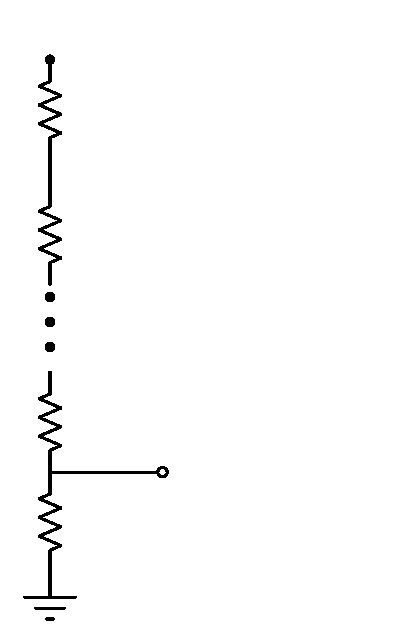
\includegraphics[scale=1]{images/Voltagedivider.eps}\\
   % translate x=208 y=444 scale 0.38
   \putbox{0.31in}{3.87in}{1.20}{$V_{applied}$}%
   \putbox{1.06in}{1.12in}{1.20}{$V_{meaured}$}%
   } % close 'parbox'
   } % close 'scalebox'
   \vspace{-\baselineskip} % this is not necessary, but looks better

			\caption{voltage divider to measure the applied
			voltage}
		\end{figure}
		
	\item Power dissipation: it could be measured 
		\begin{equation}
			P = V_{in} \times I_{in}
		\end{equation}
		where $V_{in}$ is the input voltage and $I_{in}$ is the 
		input  current

	\item Thrust/Lift: Due to a lack of fine equipment the following
		method is used, we load the ionocraft with some weight and 
		when the ionocraft reaches equilibrium the weight of the 
		ionocraft is measured using a sensitive scale.

	\item gap distance: since the gap distance measured in
		centimeters, it is safe to measure it using a regular ruler.
		
\end{enumerate}
\subsection*{Experiment Setup:}
\begin{enumerate}
	\item Setup 1:\\
	In Setup 1, we prepared a Triangular ionocraft with a side length
	10 cm, and aluminum foil height of 4cm,
	with wooden skewers as support.
	The voltage applied $\approx 30KV$ (we couldn't measure it
	accurately due to the loading effect, but the arc established at
	around 1cm).
	Unfortunately, the ionocraft didn't fly, the ionocraft was too
	heavy to take off, and the thrust was too weak.
	First, we try to increase the input voltage from 12 volts up
	to 19 volts, but unfortunately, the thrust was too weak to make
	the ionocraft fly, we couldn't measure the thrust of
	due to a lack of equipment and the ionocraft is still fixed.

\begin{figure}[ht]
	\centering
	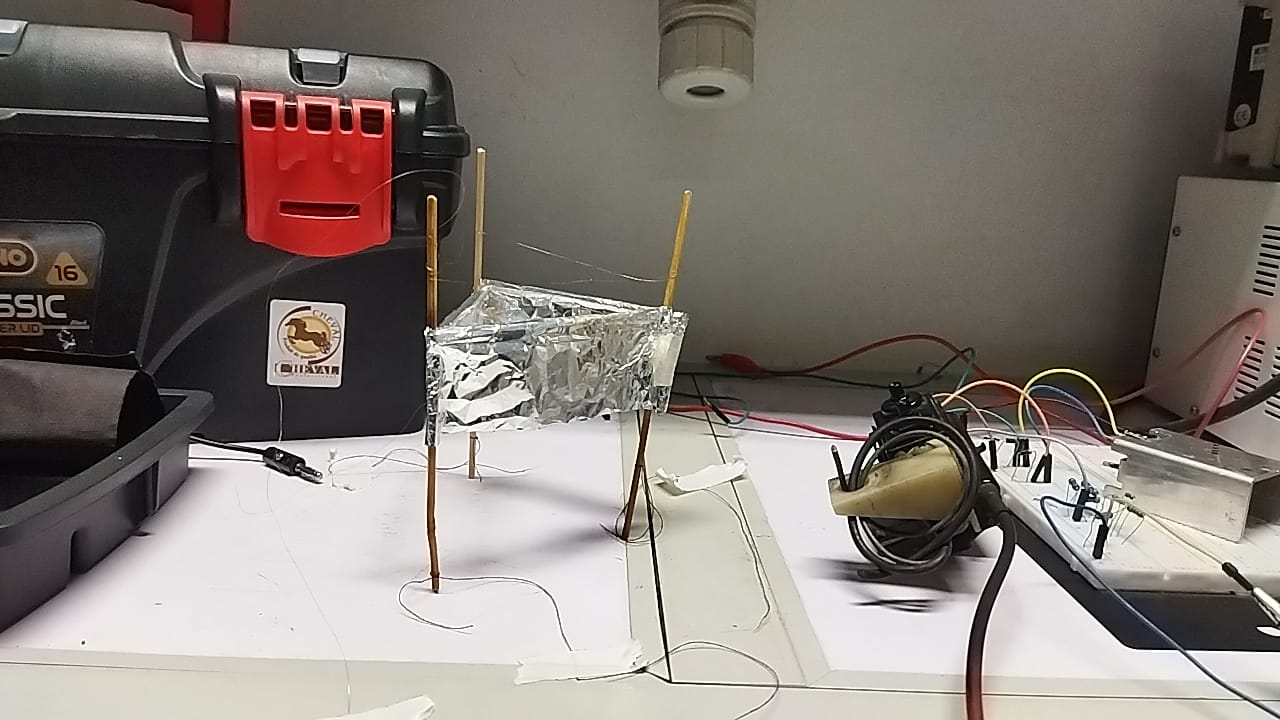
\includegraphics[scale=0.3]{images/results images/setup1.jpeg}
	\caption{Setup 1 Triangular ionocraft with wooden skewers
	support}
\end{figure}

	\item Setup 2:\\
	In this setup we made the following changes: the wooden
	skewers were replaced by plastic straws, the length
	of the support was reduced, and the height of the aluminum foil
	was reduced ( and unfortunately not measured), and third the input
	voltage was increased to 30 volts.\\
	Unfortunately, the ionocraft didn't fly, and the thrust was
	stronger(and again not measured as the ionocraft was standstill
	).
	\newpage
	Now, we may make changes to the circuit generating the High
	voltage itself, we plan to make the ionocraft lighter
	and the collector smoother
	or worst case change the structure itself.
	We should also change the measuring technique, to allow for
	measuring weak Lifts even when the ionocraft is on the ground.
	\begin{figure}[ht]
		\centering
		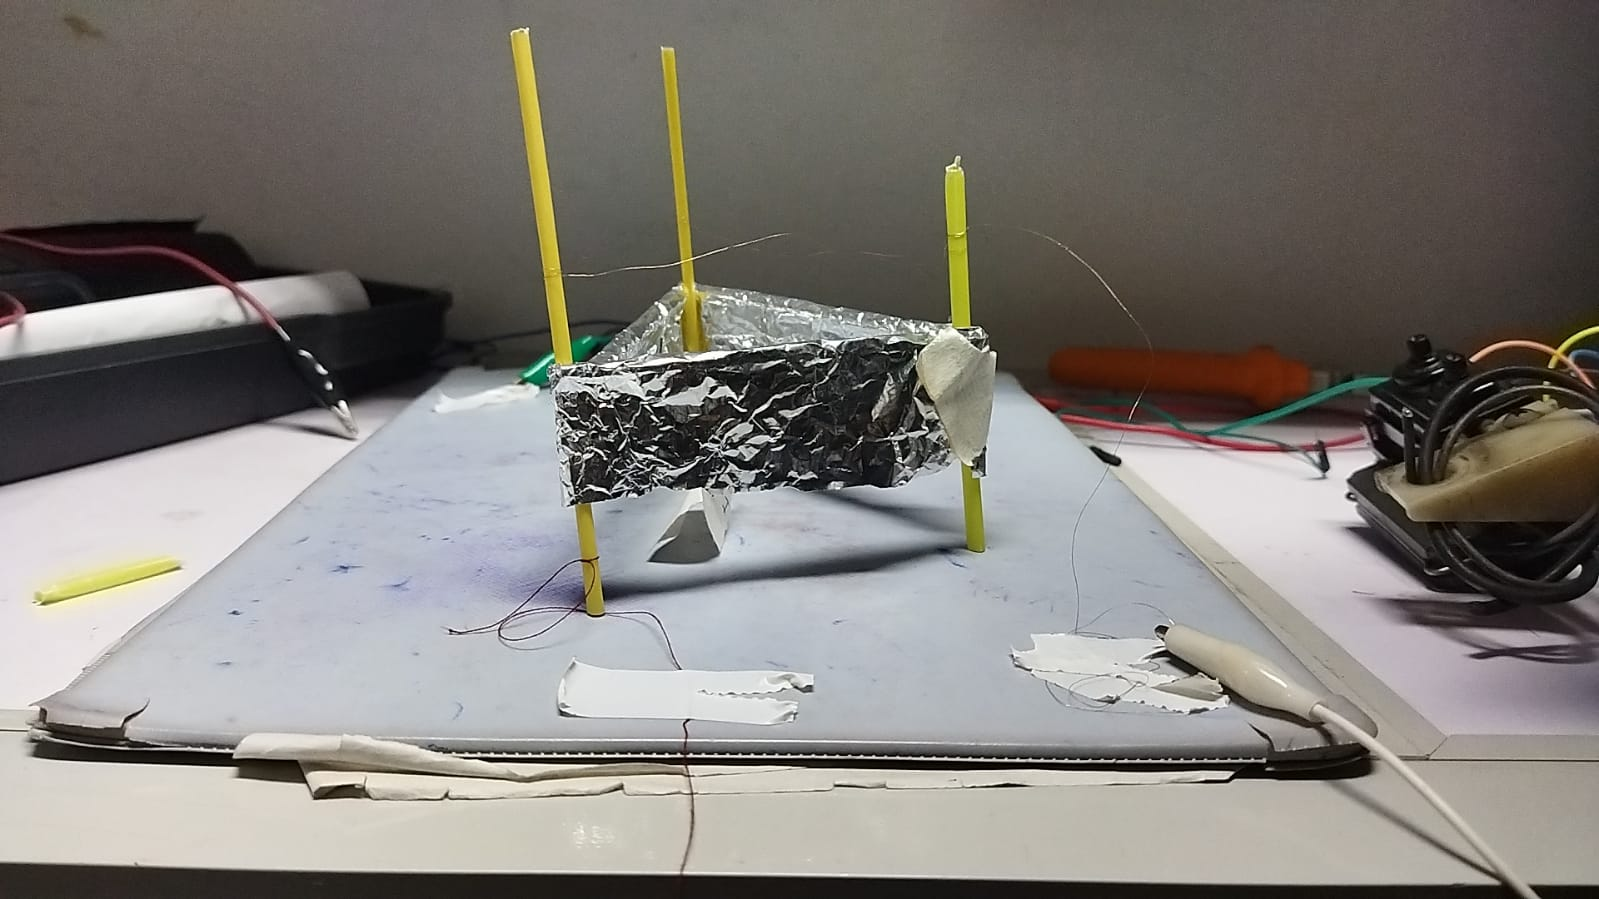
\includegraphics[scale =0.27]{images/results images/setup2.jpeg}
		\caption{Setup 2 Triangular ionocraft with plastic straws}
	\end{figure}

	For now, we will use another Experiment data to test the models.
\end{enumerate}



\section*{Simulating the model using CST}
\hspace{\parindent}This method is being mentioned just to record the numerous tries we made to use this software (CST), but all of it came to a bad end.
\begin{enumerate}
    \item We started to draw the unit of the lifter wire and the aluminum foil
    \item We can’t set voltage to a non-PEC martial 
    \item We set both the wire and aluminum foil into PEC and imagine it as an approximation 
    \item We take the steps into initializing the system and boundary conditions.
    \item due to limited knowledge and time when simulating no results output because of an error that connects the two PEC
\end{enumerate}

\section*{Simulating the model using Comsol}
\hspace{\parindent} Simulating the model using the Corona discharge previously defined package in Comsol was somehow a challenging task, but we could get some results as we did the following:
\begin{enumerate}
    \item Studying the plasma module (the module specified to simulate corona discharge)
    \item Defining the constants and parameters usually used in the simulation
    \item Setting all the required chemical reactions, including:
            \begin{enumerate}
                \item Electron impact reactions
                \item Surface reactions
                
            \end{enumerate}
    \item Setting the initial values 
    \item Setting the boundary conditions 
    \item Adjusting the meshing to solve by finite volume method (which is preferable for the software)
    \item Adjusting time dependency to take results in different instants
    
\end{enumerate}
\hspace{\parindent}After all of this, we could get results, but what was disappointing is that we couldn't get results except for the 1D model, as the other 2D and 3D models have failed due to both technical and informatics problems.
\hspace{\parindent}From these results, we could calculate the current density at the applied voltage we did in the hardware and got to compare them in the analysis section.

\subsubsection*{Results of the simulation}
\begin{figure}[p]
	\centering
	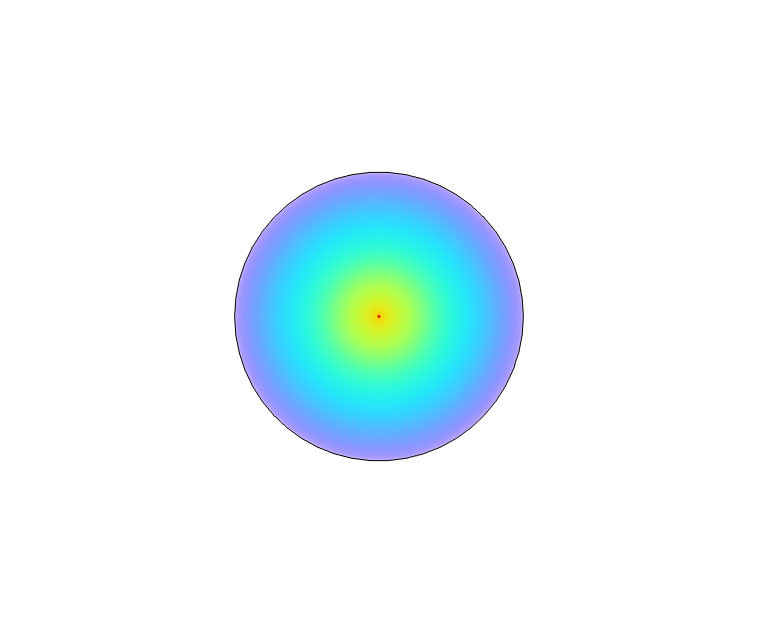
\includegraphics[scale=0.3]{images/results images/Comsol images/log of positive ion density.png}
	\caption{log of positive ion density}
\end{figure}
\begin{figure}[p]
	\centering
	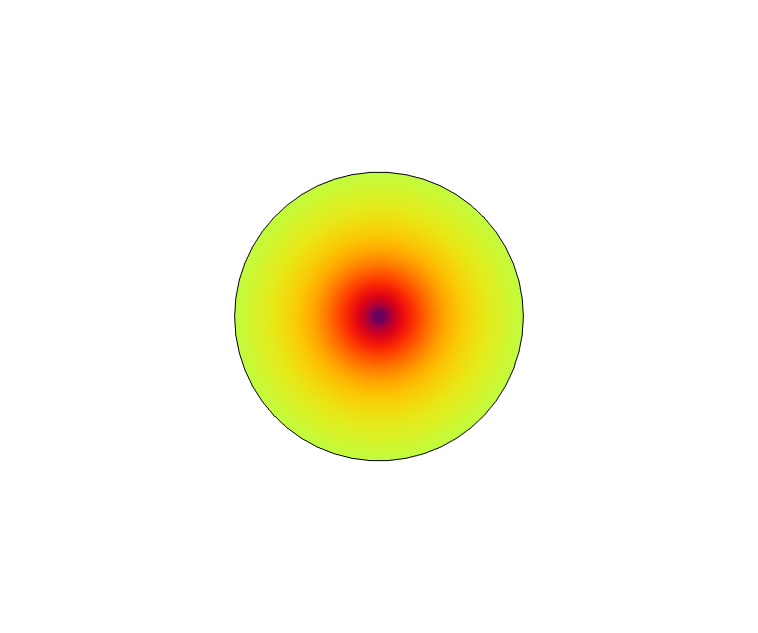
\includegraphics[scale=0.4]{images/results images/Comsol images/log of negative ion density.png}
	\caption{log of negative ion density
	support}
\end{figure}
\begin{figure}[p]
	\centering
	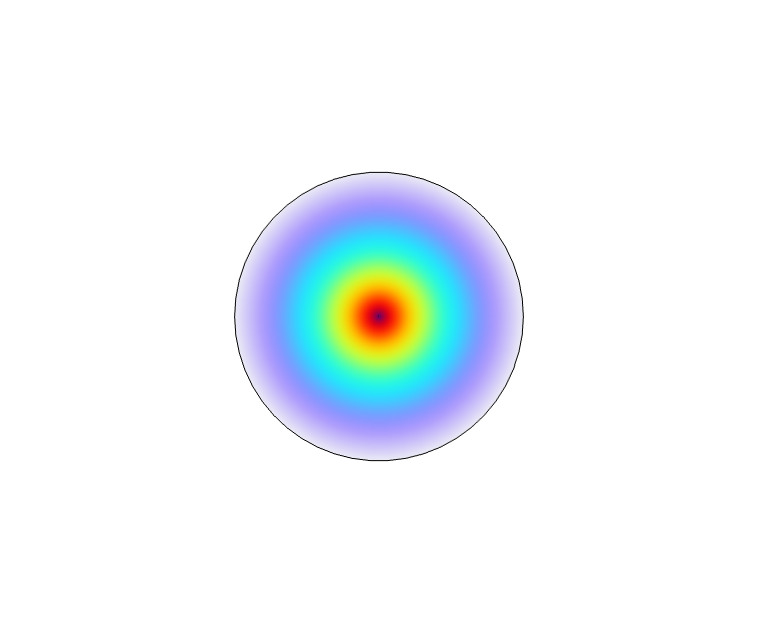
\includegraphics[scale=0.4]{images/results images/Comsol images/log of electron density.png}
	\caption{log of electron density
	support}
\end{figure}

\begin{figure}[p]
	\centering
	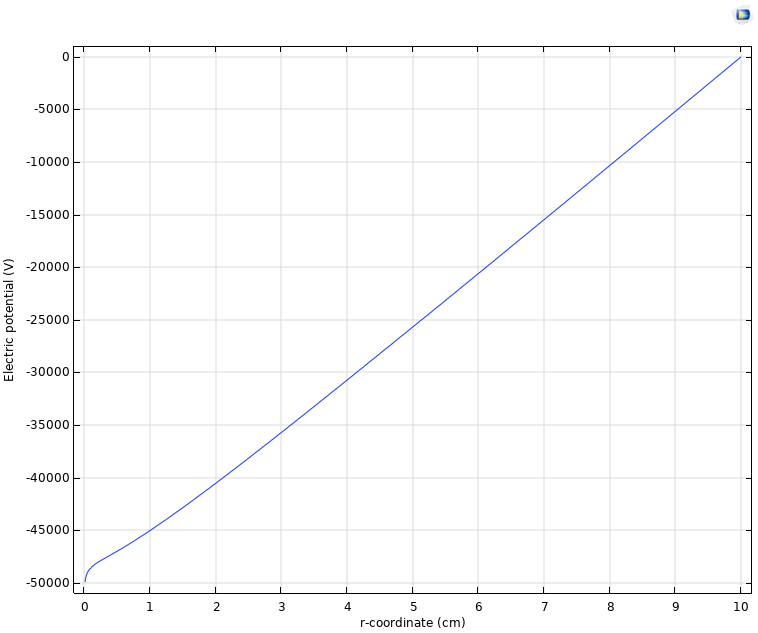
\includegraphics[scale=0.25]{images/results images/Comsol images/Electric potential.png}
	\caption{Electric potential vs r coordinate
	support}
\end{figure}

\begin{figure}[p]
	\centering
	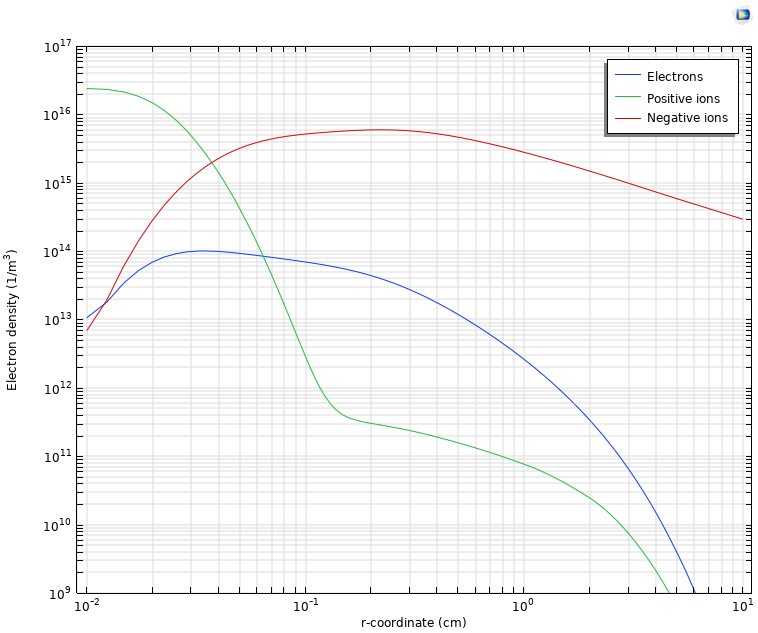
\includegraphics[scale=0.25]{images/results images/Comsol images/Electron density.png}
	\caption{Electron density vs r coordinate
	support}
\end{figure}


\begin{figure}[p]
	\centering
	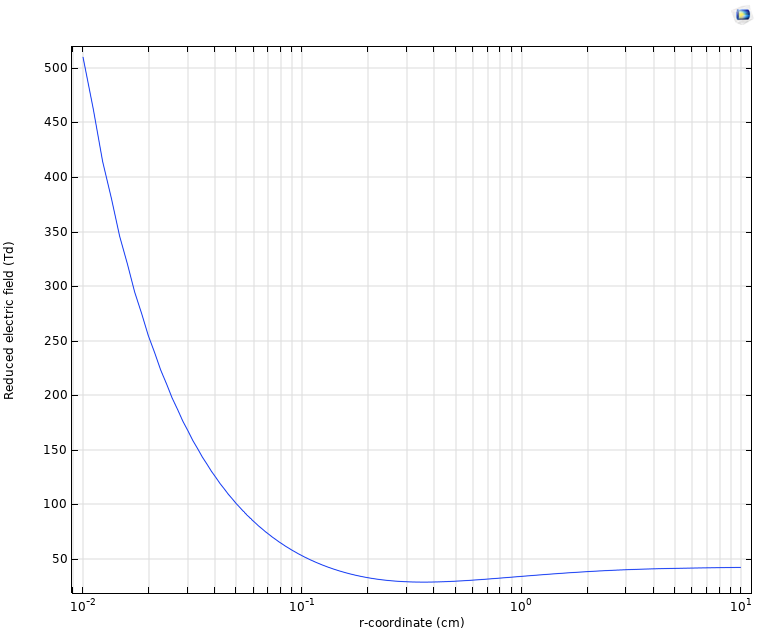
\includegraphics[scale=0.25]{images/results images/Comsol images/reduced electric field.png}
	\caption{Reduced electric field vs r coordinate
	support}
\end{figure}
\begin{figure}[p]
	\centering
	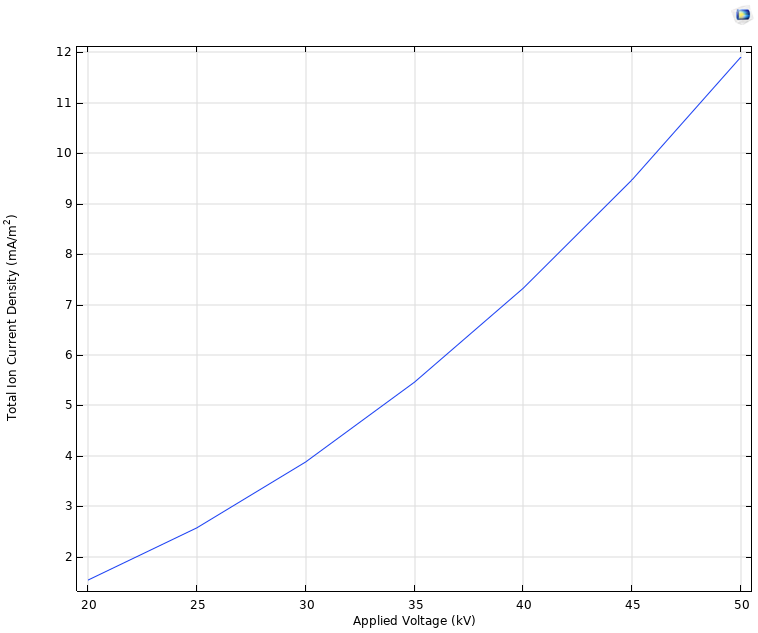
\includegraphics[scale=0.25]{images/results images/Comsol images/total ion current density.png}
	\caption{Total ion current density vs applied voltage
	support}
\end{figure}

\newpage
\section*{Solving the equations using Matlab}
\hspace{\parindent}As mentioned before our aim is to solve the equations of the second “real model” and to find the voltage distribution and field intensity everywhere, and of course, to find the velocity of air of the unit we aim to model, so we tried to solve it using Matlab packages and its numerical methods.
\subsection*{The flow of the algorithm}
The flow can be described as follows:
\begin{enumerate}
    \item Defining the parameters we need most important that were mentioned before like permittivity and geometry parameters
    \item Setting the boundary conditions of the second model, as we use the numerical method of (finite difference) to solve all the equations together
    \item  Identifying the grid and mesh
    \item Starting with the initial condition to solve Poisson getting the voltage everywhere
    \item Entering a loop to get better accuracy
    \item Calculating electric field created on the ions
    \item Calculating the velocity to be able to calculate the thrust ("but at this point it was a little hard to get good results at Matlab")
\end{enumerate}
\begin{figure}[ht]
	\centering
	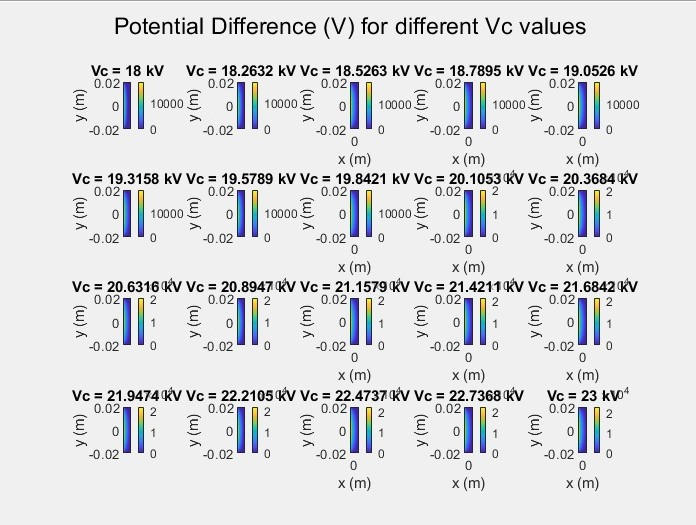
\includegraphics[scale=0.8]{images/results images/matlab images/potential Difference.jpeg}
	\caption{Potential Difference for different applied voltages}
        \vspace*{\floatsep}
        
        	\centering
        	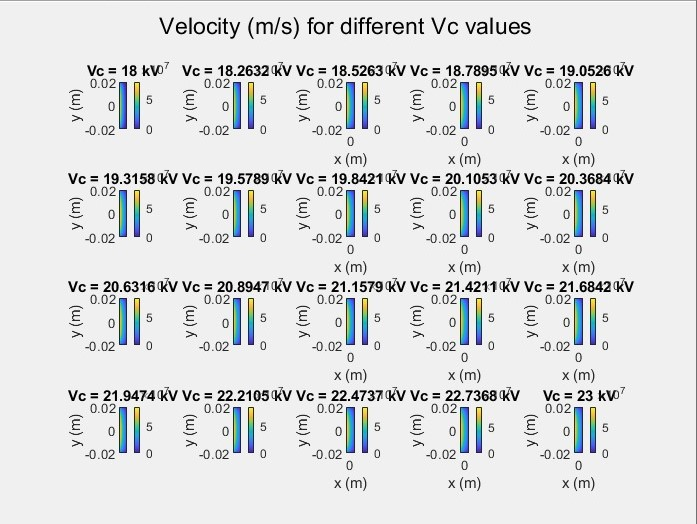
\includegraphics[scale=0.8]{images/results images/matlab images/velocity (2).jpeg}
        	\caption{Velocity intensity for different applied voltages }
        \end{figure}
        




\pagebreak
\bibliographystyle{unsrtnat}
%\bibliography{references/modelling_references}%add your refrences to this file
%\myframe
\end{document}
